% GNUPLOT: LaTeX picture with Postscript
\begingroup
  \makeatletter
  \providecommand\color[2][]{%
    \GenericError{(gnuplot) \space\space\space\@spaces}{%
      Package color not loaded in conjunction with
      terminal option `colourtext'%
    }{See the gnuplot documentation for explanation.%
    }{Either use 'blacktext' in gnuplot or load the package
      color.sty in LaTeX.}%
    \renewcommand\color[2][]{}%
  }%
  \providecommand\includegraphics[2][]{%
    \GenericError{(gnuplot) \space\space\space\@spaces}{%
      Package graphicx or graphics not loaded%
    }{See the gnuplot documentation for explanation.%
    }{The gnuplot epslatex terminal needs graphicx.sty or graphics.sty.}%
    \renewcommand\includegraphics[2][]{}%
  }%
  \providecommand\rotatebox[2]{#2}%
  \@ifundefined{ifGPcolor}{%
    \newif\ifGPcolor
    \GPcolortrue
  }{}%
  \@ifundefined{ifGPblacktext}{%
    \newif\ifGPblacktext
    \GPblacktexttrue
  }{}%
  % define a \g@addto@macro without @ in the name:
  \let\gplgaddtomacro\g@addto@macro
  % define empty templates for all commands taking text:
  \gdef\gplbacktext{}%
  \gdef\gplfronttext{}%
  \makeatother
  \ifGPblacktext
    % no textcolor at all
    \def\colorrgb#1{}%
    \def\colorgray#1{}%
  \else
    % gray or color?
    \ifGPcolor
      \def\colorrgb#1{\color[rgb]{#1}}%
      \def\colorgray#1{\color[gray]{#1}}%
      \expandafter\def\csname LTw\endcsname{\color{white}}%
      \expandafter\def\csname LTb\endcsname{\color{black}}%
      \expandafter\def\csname LTa\endcsname{\color{black}}%
      \expandafter\def\csname LT0\endcsname{\color[rgb]{1,0,0}}%
      \expandafter\def\csname LT1\endcsname{\color[rgb]{0,1,0}}%
      \expandafter\def\csname LT2\endcsname{\color[rgb]{0,0,1}}%
      \expandafter\def\csname LT3\endcsname{\color[rgb]{1,0,1}}%
      \expandafter\def\csname LT4\endcsname{\color[rgb]{0,1,1}}%
      \expandafter\def\csname LT5\endcsname{\color[rgb]{1,1,0}}%
      \expandafter\def\csname LT6\endcsname{\color[rgb]{0,0,0}}%
      \expandafter\def\csname LT7\endcsname{\color[rgb]{1,0.3,0}}%
      \expandafter\def\csname LT8\endcsname{\color[rgb]{0.5,0.5,0.5}}%
    \else
      % gray
      \def\colorrgb#1{\color{black}}%
      \def\colorgray#1{\color[gray]{#1}}%
      \expandafter\def\csname LTw\endcsname{\color{white}}%
      \expandafter\def\csname LTb\endcsname{\color{black}}%
      \expandafter\def\csname LTa\endcsname{\color{black}}%
      \expandafter\def\csname LT0\endcsname{\color{black}}%
      \expandafter\def\csname LT1\endcsname{\color{black}}%
      \expandafter\def\csname LT2\endcsname{\color{black}}%
      \expandafter\def\csname LT3\endcsname{\color{black}}%
      \expandafter\def\csname LT4\endcsname{\color{black}}%
      \expandafter\def\csname LT5\endcsname{\color{black}}%
      \expandafter\def\csname LT6\endcsname{\color{black}}%
      \expandafter\def\csname LT7\endcsname{\color{black}}%
      \expandafter\def\csname LT8\endcsname{\color{black}}%
    \fi
  \fi
    \setlength{\unitlength}{0.0500bp}%
    \ifx\gptboxheight\undefined%
      \newlength{\gptboxheight}%
      \newlength{\gptboxwidth}%
      \newsavebox{\gptboxtext}%
    \fi%
    \setlength{\fboxrule}{0.5pt}%
    \setlength{\fboxsep}{1pt}%
\begin{picture}(14400.00,5760.00)%
    \gplgaddtomacro\gplbacktext{%
      \csname LTb\endcsname%%
      \put(618,1038){\makebox(0,0)[r]{\strut{}\np{e-4}}}%
      \csname LTb\endcsname%%
      \put(618,1812){\makebox(0,0)[r]{\strut{}\np{e-2}}}%
      \csname LTb\endcsname%%
      \put(618,2586){\makebox(0,0)[r]{\strut{}\np{1}}}%
      \csname LTb\endcsname%%
      \put(618,3359){\makebox(0,0)[r]{\strut{}\np{e2}}}%
      \csname LTb\endcsname%%
      \put(618,4133){\makebox(0,0)[r]{\strut{}\np{e4}}}%
      \csname LTb\endcsname%%
      \put(618,4907){\makebox(0,0)[r]{\strut{}\np{e6}}}%
      \csname LTb\endcsname%%
      \put(1100,465){\makebox(0,0){\strut{}\np{e-4}}}%
      \csname LTb\endcsname%%
      \put(1860,465){\makebox(0,0){\strut{}\np{e-2}}}%
      \csname LTb\endcsname%%
      \put(2620,465){\makebox(0,0){\strut{}1}}%
      \csname LTb\endcsname%%
      \put(3379,465){\makebox(0,0){\strut{}\np{e2}}}%
      \csname LTb\endcsname%%
      \put(4139,465){\makebox(0,0){\strut{}\np{e4}}}%
      \csname LTb\endcsname%%
      \put(4899,465){\makebox(0,0){\strut{}\np{e6}}}%
    }%
    \gplgaddtomacro\gplfronttext{%
      \csname LTb\endcsname%%
      \put(126,2972){\rotatebox{-270}{\makebox(0,0){\strut{}Cross-section (b)}}}%
      \csname LTb\endcsname%%
      \put(2999,186){\makebox(0,0){\strut{}Energy (eV)}}%
      \csname LTb\endcsname%%
      \put(2999,5573){\makebox(0,0){\strut{}Hydrogen \tapi{1}H}}%
      \csname LTb\endcsname%%
      \put(4746,5127){\makebox(0,0)[r]{\strut{}Total}}%
      \csname LTb\endcsname%%
      \put(4746,4941){\makebox(0,0)[r]{\strut{}Elastic}}%
      \csname LTb\endcsname%%
      \put(4746,4755){\makebox(0,0)[r]{\strut{}Capture}}%
      \csname LTb\endcsname%%
      \put(618,1038){\makebox(0,0)[r]{\strut{}\np{e-4}}}%
      \csname LTb\endcsname%%
      \put(618,1812){\makebox(0,0)[r]{\strut{}\np{e-2}}}%
      \csname LTb\endcsname%%
      \put(618,2586){\makebox(0,0)[r]{\strut{}1}}%
      \csname LTb\endcsname%%
      \put(618,3359){\makebox(0,0)[r]{\strut{}\np{e2}}}%
      \csname LTb\endcsname%%
      \put(618,4133){\makebox(0,0)[r]{\strut{}\np{e4}}}%
      \csname LTb\endcsname%%
      \put(618,4907){\makebox(0,0)[r]{\strut{}\np{e6}}}%
      \csname LTb\endcsname%%
      \put(1100,465){\makebox(0,0){\strut{}\np{e-4}}}%
      \csname LTb\endcsname%%
      \put(1860,465){\makebox(0,0){\strut{}\np{e-2}}}%
      \csname LTb\endcsname%%
      \put(2620,465){\makebox(0,0){\strut{}1}}%
      \csname LTb\endcsname%%
      \put(3379,465){\makebox(0,0){\strut{}\np{e2}}}%
      \csname LTb\endcsname%%
      \put(4139,465){\makebox(0,0){\strut{}\np{e4}}}%
      \csname LTb\endcsname%%
      \put(4899,465){\makebox(0,0){\strut{}\np{e6}}}%
    }%
    \gplgaddtomacro\gplbacktext{%
      \csname LTb\endcsname%%
      \put(5178,1038){\makebox(0,0)[r]{\strut{}}}%
      \csname LTb\endcsname%%
      \put(5178,1812){\makebox(0,0)[r]{\strut{}}}%
      \csname LTb\endcsname%%
      \put(5178,2586){\makebox(0,0)[r]{\strut{}}}%
      \csname LTb\endcsname%%
      \put(5178,3359){\makebox(0,0)[r]{\strut{}}}%
      \csname LTb\endcsname%%
      \put(5178,4133){\makebox(0,0)[r]{\strut{}}}%
      \csname LTb\endcsname%%
      \put(5178,4907){\makebox(0,0)[r]{\strut{}}}%
      \csname LTb\endcsname%%
      \put(5280,465){\makebox(0,0){\strut{}\np{e-5}}}%
      \csname LTb\endcsname%%
      \put(6036,465){\makebox(0,0){\strut{}\np{e-4}}}%
      \csname LTb\endcsname%%
      \put(6791,465){\makebox(0,0){\strut{}\np{e-3}}}%
      \csname LTb\endcsname%%
      \put(7547,465){\makebox(0,0){\strut{}\np{e-2}}}%
      \csname LTb\endcsname%%
      \put(8303,465){\makebox(0,0){\strut{}\np{0.1}}}%
      \csname LTb\endcsname%%
      \put(9058,465){\makebox(0,0){\strut{}\np{1}}}%
      \csname LTb\endcsname%%
      \put(9814,465){\makebox(0,0){\strut{}10}}%
      \csname LTb\endcsname%%
      \put(10570,465){\makebox(0,0){\strut{}\np{e2}}}%
      \csname LTb\endcsname%%
      \put(11325,465){\makebox(0,0){\strut{}\np{e3}}}%
      \csname LTb\endcsname%%
      \put(12081,465){\makebox(0,0){\strut{}\np{e4}}}%
      \csname LTb\endcsname%%
      \put(12837,465){\makebox(0,0){\strut{}\np{e5}}}%
      \csname LTb\endcsname%%
      \put(13592,465){\makebox(0,0){\strut{}\np{e6}}}%
      \csname LTb\endcsname%%
      \put(14348,465){\makebox(0,0){\strut{}\np{e7}}}%
    }%
    \gplgaddtomacro\gplfronttext{%
      \csname LTb\endcsname%%
      \put(5178,2972){\rotatebox{-270}{\makebox(0,0){\strut{}}}}%
      \csname LTb\endcsname%%
      \put(9814,186){\makebox(0,0){\strut{}Energy (eV)}}%
      \csname LTb\endcsname%%
      \put(9814,5573){\makebox(0,0){\strut{}Gadolinium \tapi{157}Gd}}%
      \csname LTb\endcsname%%
      \put(13815,5127){\makebox(0,0)[r]{\strut{}Total}}%
      \csname LTb\endcsname%%
      \put(13815,4941){\makebox(0,0)[r]{\strut{}Elastic}}%
      \csname LTb\endcsname%%
      \put(13815,4755){\makebox(0,0)[r]{\strut{}Capture}}%
      \csname LTb\endcsname%%
      \put(5178,1038){\makebox(0,0)[r]{\strut{}}}%
      \csname LTb\endcsname%%
      \put(5178,1812){\makebox(0,0)[r]{\strut{}}}%
      \csname LTb\endcsname%%
      \put(5178,2586){\makebox(0,0)[r]{\strut{}}}%
      \csname LTb\endcsname%%
      \put(5178,3359){\makebox(0,0)[r]{\strut{}}}%
      \csname LTb\endcsname%%
      \put(5178,4133){\makebox(0,0)[r]{\strut{}}}%
      \csname LTb\endcsname%%
      \put(5178,4907){\makebox(0,0)[r]{\strut{}}}%
      \csname LTb\endcsname%%
      \put(5280,465){\makebox(0,0){\strut{}\np{e-5}}}%
      \csname LTb\endcsname%%
      \put(6036,465){\makebox(0,0){\strut{}\np{e-4}}}%
      \csname LTb\endcsname%%
      \put(6791,465){\makebox(0,0){\strut{}\np{e-3}}}%
      \csname LTb\endcsname%%
      \put(7547,465){\makebox(0,0){\strut{}\np{e-2}}}%
      \csname LTb\endcsname%%
      \put(8303,465){\makebox(0,0){\strut{}\np{0.1}}}%
      \csname LTb\endcsname%%
      \put(9058,465){\makebox(0,0){\strut{}\np{1}}}%
      \csname LTb\endcsname%%
      \put(9814,465){\makebox(0,0){\strut{}\np{10}}}%
      \csname LTb\endcsname%%
      \put(10570,465){\makebox(0,0){\strut{}\np{e2}}}%
      \csname LTb\endcsname%%
      \put(11325,465){\makebox(0,0){\strut{}\np{e3}}}%
      \csname LTb\endcsname%%
      \put(12081,465){\makebox(0,0){\strut{}\np{e4}}}%
      \csname LTb\endcsname%%
      \put(12837,465){\makebox(0,0){\strut{}\np{e5}}}%
      \csname LTb\endcsname%%
      \put(13592,465){\makebox(0,0){\strut{}\np{e6}}}%
      \csname LTb\endcsname%%
      \put(14348,465){\makebox(0,0){\strut{}\np{e7}}}%
    }%
    \iffalse
    \gplgaddtomacro\gplbacktext{%
      \csname LTb\endcsname%%
      \put(8717,864){\makebox(0,0)[l]{\strut{}0.1}}%
      \csname LTb\endcsname%%
      \put(8717,1382){\makebox(0,0)[l]{\strut{}1}}%
      \csname LTb\endcsname%%
      \put(8717,1900){\makebox(0,0)[l]{\strut{}10}}%
      \csname LTb\endcsname%%
      \put(8717,2419){\makebox(0,0)[l]{\strut{}\np{e2}}}%
      \csname LTb\endcsname%%
      \put(8717,2937){\makebox(0,0)[l]{\strut{}\np{e3}}}%
      \csname LTb\endcsname%%
      \put(8717,3455){\makebox(0,0)[l]{\strut{}\np{e4}}}%
      \csname LTb\endcsname%%
      \put(5989,3641){\makebox(0,0){\strut{}20}}%
      \csname LTb\endcsname%%
      \put(6737,3641){\makebox(0,0){\strut{}50}}%
      \csname LTb\endcsname%%
      \put(7868,3641){\makebox(0,0){\strut{}200}}%
      \csname LTb\endcsname%%
      \put(8615,3641){\makebox(0,0){\strut{}500}}%
      \csname LTb\endcsname%%
      \put(5424,3641){\makebox(0,0){\strut{}10}}%
      \csname LTb\endcsname%%
      \put(7302,3641){\makebox(0,0){\strut{}100}}%
    }%
    \fi
    \gplgaddtomacro\gplfronttext{%
      \csname LTb\endcsname%%
      \put(5433,2159){\rotatebox{-270}{\makebox(0,0){\strut{}}}}%
      \csname LTb\endcsname%%
      \put(7019,808){\makebox(0,0){\strut{}}}%
      \csname LTb\endcsname%%
      \put(7019,3548){\makebox(0,0){\strut{}}}%
      \csname LTb\endcsname%%
      \put(8717,864){\makebox(0,0)[l]{\strut{}0.1}}%
      \csname LTb\endcsname%%
      \put(8717,1382){\makebox(0,0)[l]{\strut{}1}}%
      \csname LTb\endcsname%%
      \put(8717,1900){\makebox(0,0)[l]{\strut{}10}}%
      \csname LTb\endcsname%%
      \put(8717,2419){\makebox(0,0)[l]{\strut{}\np{e2}}}%
      \csname LTb\endcsname%%
      \put(8717,2937){\makebox(0,0)[l]{\strut{}\np{e3}}}%
      \csname LTb\endcsname%%
      \put(8717,3455){\makebox(0,0)[l]{\strut{}\np{e4}}}%
      \csname LTb\endcsname%%
      \put(5989,3641){\makebox(0,0){\strut{}20}}%
      \csname LTb\endcsname%%
      \put(6737,3641){\makebox(0,0){\strut{}50}}%
      \csname LTb\endcsname%%
      \put(7868,3641){\makebox(0,0){\strut{}200}}%
      \csname LTb\endcsname%%
      \put(8615,3641){\makebox(0,0){\strut{}500}}%
      \csname LTb\endcsname%%
      \put(5424,3641){\makebox(0,0){\strut{}10}}%
      \csname LTb\endcsname%%
      \put(7302,3641){\makebox(0,0){\strut{}100}}%
    }%
    \gplbacktext
    \put(0,0){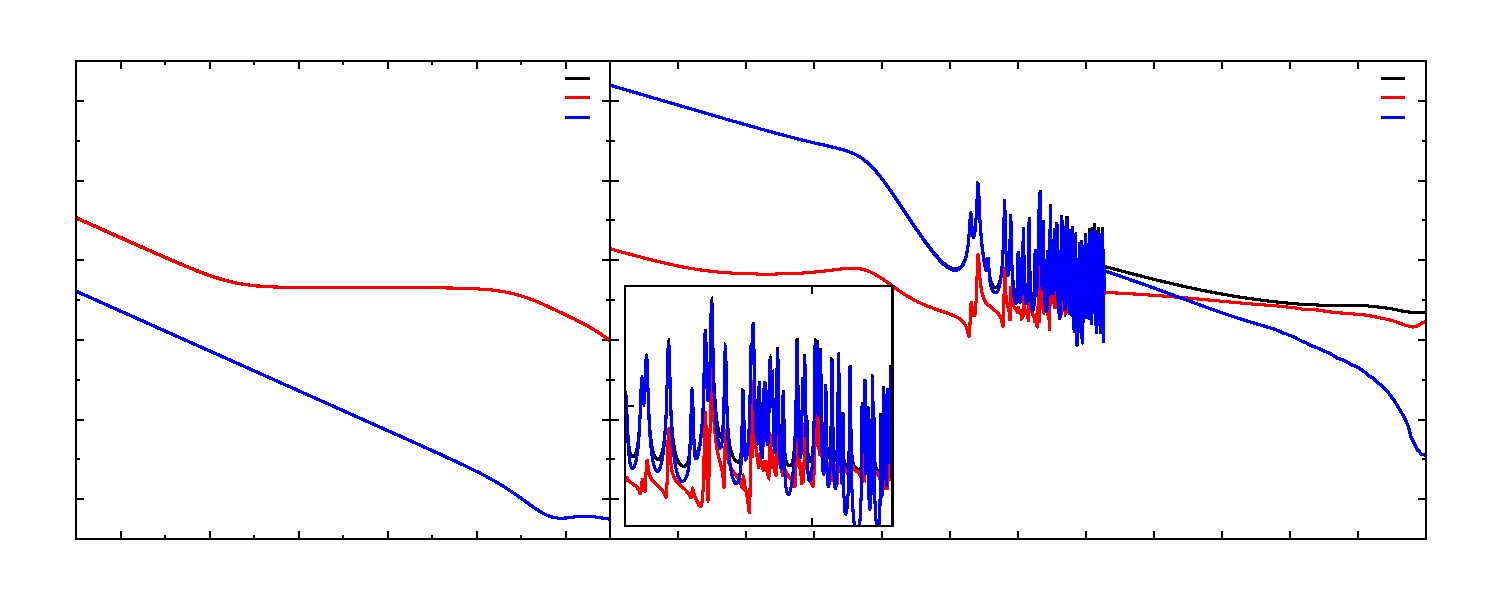
\includegraphics{pics/neutron_xsec}}%
    \gplfronttext
  \end{picture}%
\endgroup
